%%%%%%%%%%%%%%%%%%%%%%% file template.tex %%%%%%%%%%%%%%%%%%%%%%%%%
% $Id: woc_2col.tex 158 2017-01-19 23:08:23Z foley $
% $URL: https://repository.cs.ru.is/svn/template/tvd/journal/matec-woc/woc_2col.tex $
% 
% This is a template file for Web of Conferences Journal
%
% Copy it to a new file with a new name and use it as the basis
% for your article
%
% This template has been updated to match the Word Template's contents
% by Joseph T. Foley < foley AT RU dot IS >
%
%%%%%%%%%%%%%%%%%%%%%%%%%% EDP Science %%%%%%%%%%%%%%%%%%%%%%%%%%%%
%
%%%\documentclass[option]{webofc}
%%% "twocolumn" for typesetting an article in two columns format (default one column)
%
\documentclass[twocolumn]{webofc}
\usepackage[varg]{txfonts}   % Web of Conferences font
\usepackage{booktabs}
\usepackage{float}
\usepackage{pgfplots}
\usepackage{array} %% needed for advanced table manipulation
%% Column types from http://tex.stackexchange.com/questions/54069/table-with-text-wrapping
\newcolumntype{L}[1]{>{\raggedright\let\newline\\\arraybackslash\hspace{0pt}}m{#1}}
\newcolumntype{C}[1]{>{\centering\let\newline\\\arraybackslash\hspace{0pt}}m{#1}}
\newcolumntype{R}[1]{>{\raggedleft\let\newline\\\arraybackslash\hspace{0pt}}m{#1}}

\graphicspath{{graphics/}{graphics/arch/}{Graphics/}{./}} % Look in these folders for graphics
%
% Put here some packages required or/and some personnal commands
%
%

\begin{filecontents}{serverloads.dat}
\end{filecontents}

\begin{document}
%
    \title{Towards Practical and Scalable Strategies for the Online Load Balancing Problem in distributed systems}
%
% subtitle is optionnal
%
%%%\subtitle{Do you have a subtitle?\\ If so, write it here}

\author{\firstname{Maximilian} \lastname{Müller}\inst{1} \and
\firstname{Vivian} \lastname{Berger}\inst{1}
% etc.
}

\institute{Baden-Wuerttemberg Cooperative State University (DHBW) Heidenheim, Germany}

\abstract{%
    This paper presents a practical implementation strategy for online load balancing in distributed systems, combining dynamic load distribution with autoscaling capabilities. The proposed solution, implemented in \textit{Rust} and \textit{Docker}, offers an open-source alternative to proprietary cloud-based systems. The architecture employs a resource utilization-based distribution strategy, where \textit{worker} states are managed through a finite state automaton. A dynamic weighted load balancer model is introduced, utilizing a discrete probability distribution for server selection. The system's efficiency is evaluated through theoretical analysis and empirical data collection, demonstrating high performance in both heterogeneous and homogeneous load scenarios. Additional features include a simple caching mechanism to reduce latency and backend queries, and a robust request management system capable of handling high concurrency. The implementation leverages a dedicated \textit{Docker} network for inter-component communication and uses \textit{Redis} as a key-value store for container states and metadata. The paper concludes with a classification of the algorithm within the context of the online load balancing problem, showing competitive performance compared to established algorithms while offering improved adaptability to dynamic environments
}
%
\maketitle
%

\section{Introduction}
Efficient task distribution across resources is a fundamental concern in computer science, particularly in real-time distributed systems. In contrast to offline load balancing problems, online load balancing requires decision-making without knowledge of future task arrivals. The primary objective is to distribute the load as uniformly as possible, thereby minimizing the maximum utilization of any single resource and optimizing overall system performance.
This paper focuses on a practical implementation strategy for online load balancing in distributed systems, using a resource utilization-based distribution strategy coupled with system autoscaling capabilities. Comparable commercial systems include Amazon Web Services (AWS) Elastic Load Balancer (ELB)\cite{aws_load_balancing} and Microsoft Azure Load Balancer with Azure Autoscale\cite{azure_autoscale_overview}. In contrast to these proprietary, fee-based cloud systems, the implementation presented herein is open-source and freely accessible\footnote{https://github.com/mxmueller/RustyBalancer}. While exact implementations are not disclosed, industry information suggests AWS and Microsoft use various languages like C++, Java, Go, and C\# for their cloud services\footnote{https://docs.aws.amazon.com/cdk/v2/guide/languages.html}.
In contrast, the solution presented here is natively implemented in \textit{Rust} and \textit{Docker}, enabling autoscaling on bare metal hosts without cloud provider dependencies. \textit{Rust} offers memory safety without garbage collection, resulting in predictable performance and low latencies—critical factors for load balancers in high-load environments. The ownership model and borrowing system of \textit{Rust} facilitate thread-safe parallelization without data races, allowing efficient utilization of multi-core systems for enhanced throughput performance. \textit{Rust's} type system and compile-time checks further contribute to the reliability of the load balancing system, reducing the likelihood of runtime errors and improving overall system stability\cite{klabnik2019rust}.

\section{System Architecture and Components}
The system design is based on \textit{Docker} and \textit{Docker Compose}. Docker, an industry-standard containerization platform, encapsulates applications in isolated units for consistent cross-environment deployment\cite{docker_overview}. \textit{Docker Compose} facilitates multi-container orchestration\cite{docker_compose}.
\begin{figure}[H]
    \centering
    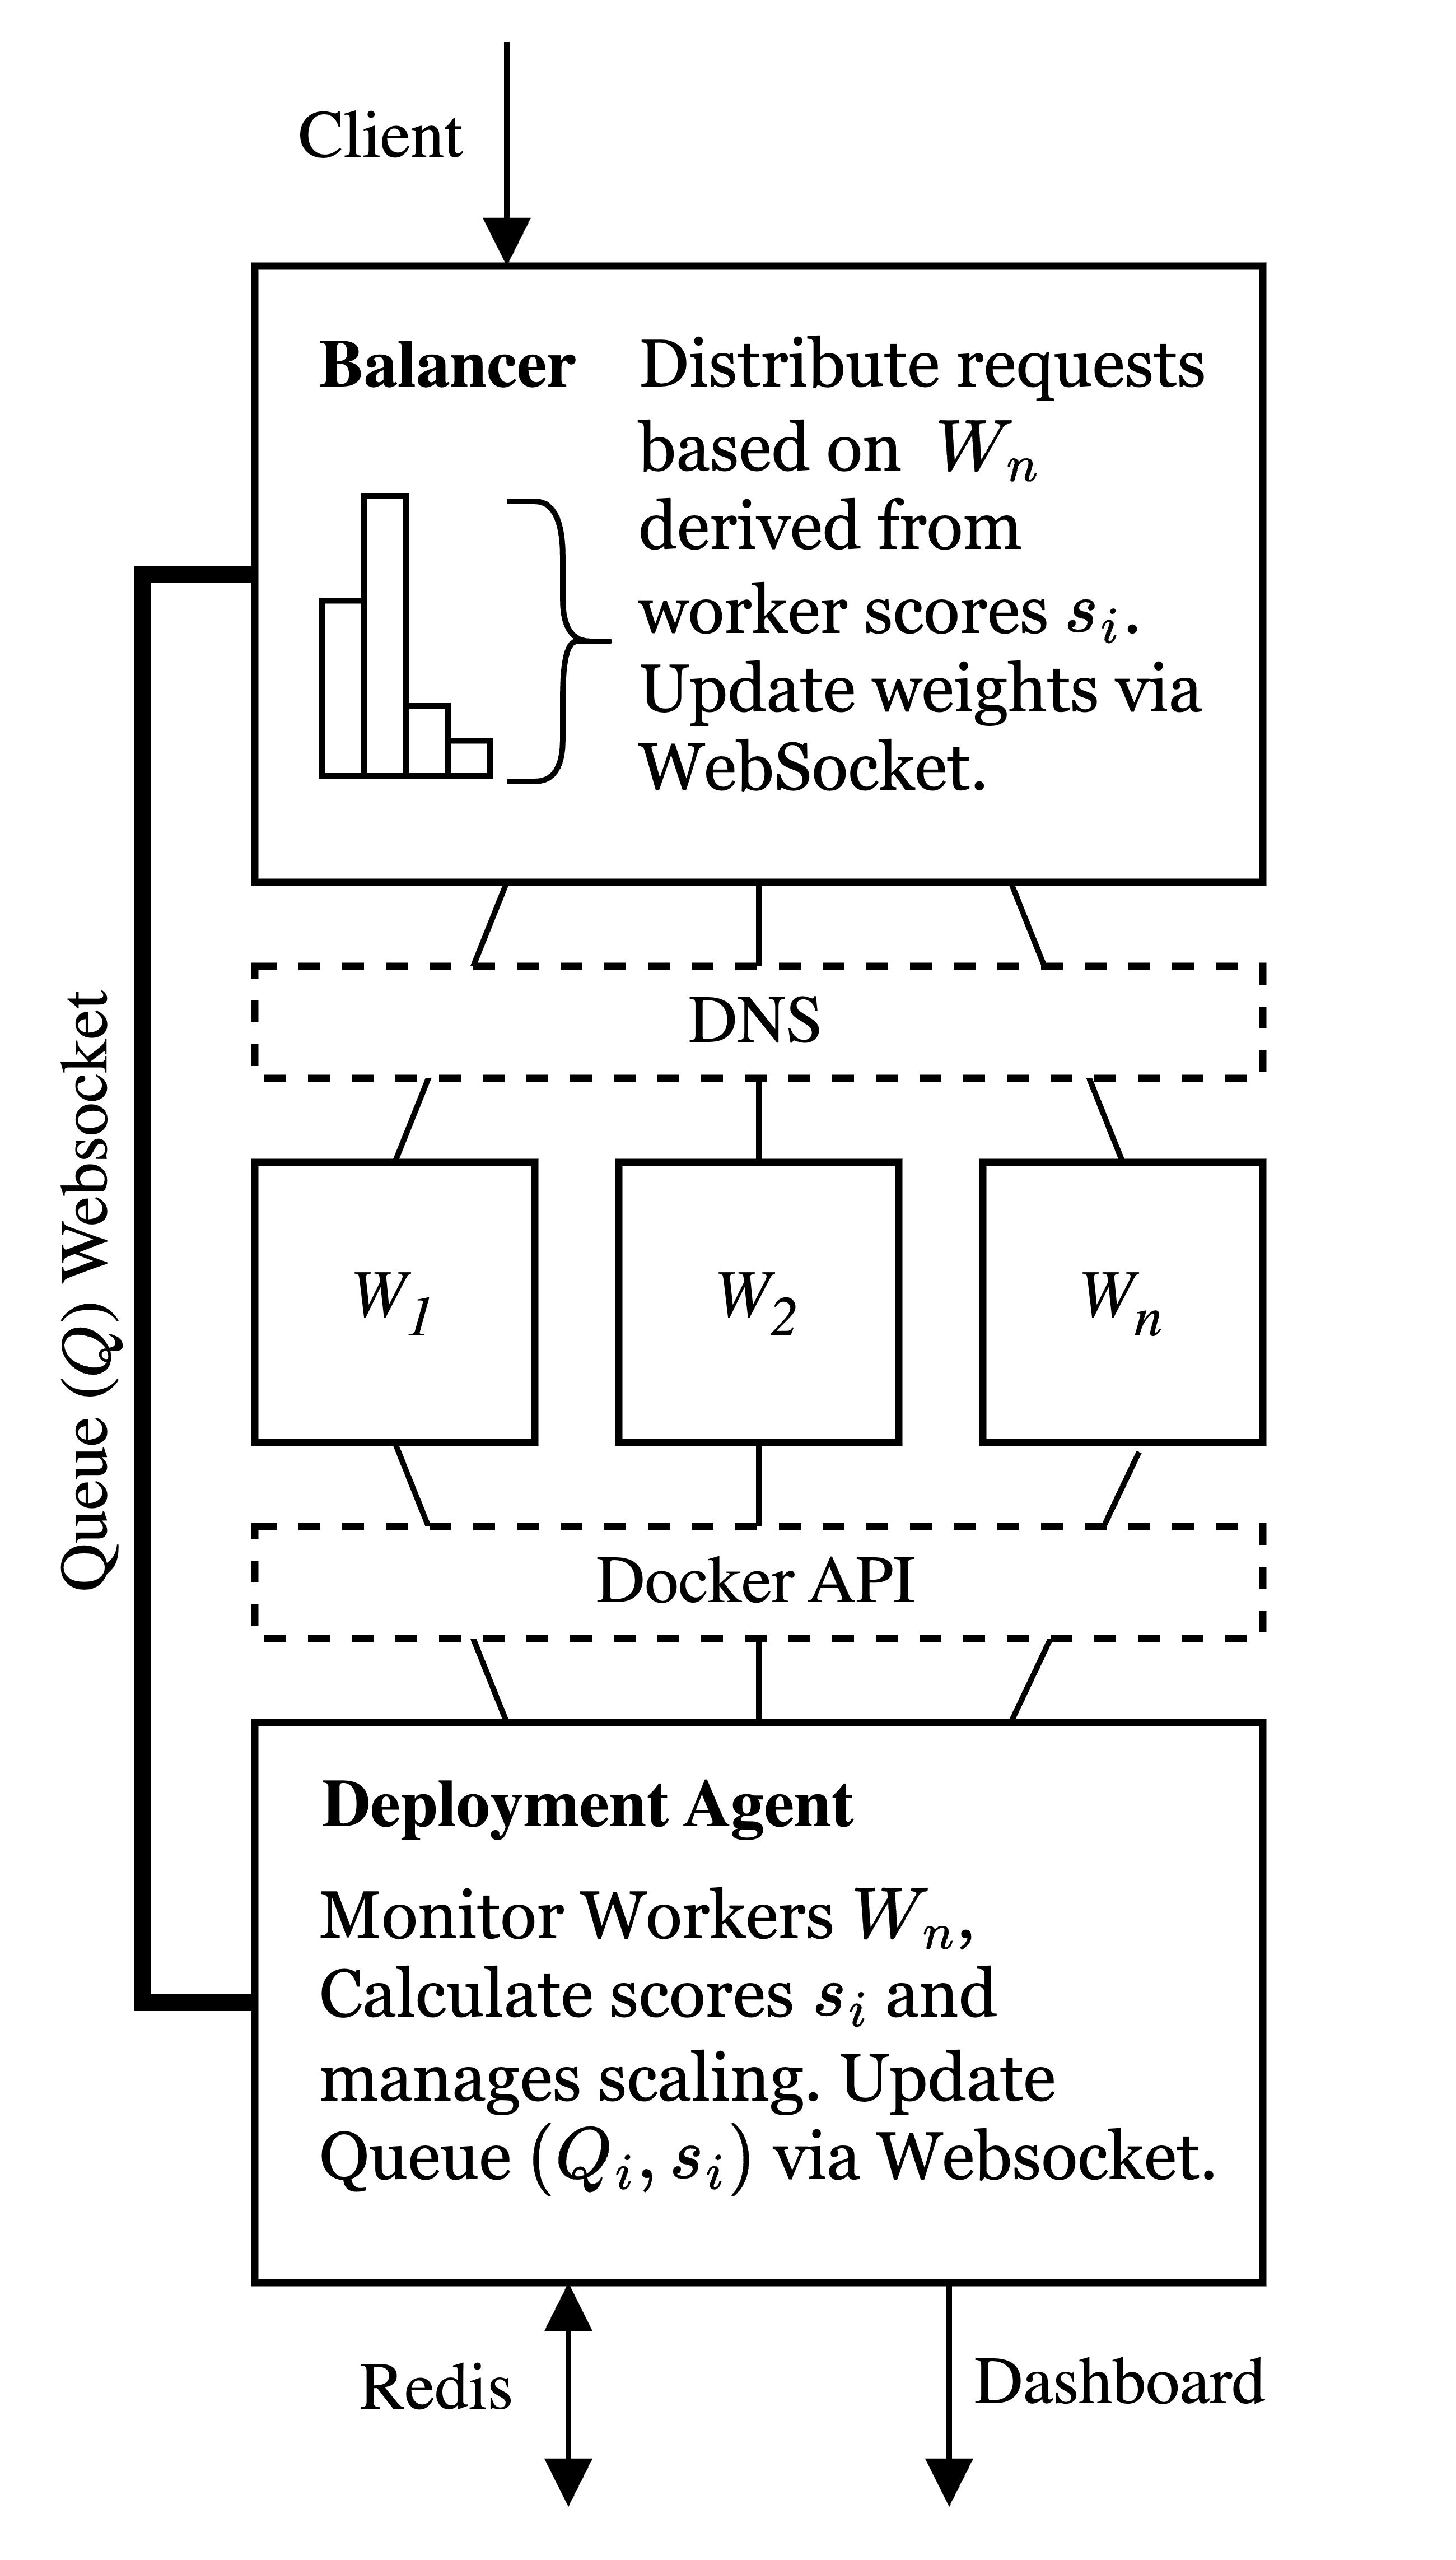
\includegraphics[width=0.701\columnwidth]{minimaloverview.png}
    \caption{This diagram provides a comprehensive overview of all components, each of which represents an active container within the system landscape established during the deployment process.}
    \label{fig:minimal}
\end{figure}
Figure~\ref{fig:minimal} serves as the foundational framework for comprehending all subsequent explanations. The architecture is derived from its task distribution. As one of the two core units, the \textit{Balancer} ensures the distribution of workload to the workers, while the interaction among workers occurs within the \textit{Deployment-Agent}. The latter will be addressed in detail in the following sections. The \textit{Worker} constitutes a fundamental operational unit within the system architecture, designed to receive and process distributed workload. This component is subject to scaling, with a minimum instantiation of one instance, and can be replicated up to the maximum capacity as determined by the host system's resource constraints. This scalability feature enables dynamic adjustment of processing capabilities in response to varying computational demands. A valid image of Docker Hub must be specified in the configuration for the resource that is made available in the \textit{Workers}.
\textit{Redis} (Remote Dictionary Server)\cite{redis_docs}, a high-performance, open-source, in-memory key-value data store, is utilized to maintain a persistent state between the currently active resources and the \textit{Workers} that are intended to be operational. This mechanism facilitates the synchronization of system state across running and desired instances, enabling efficient resource management and system consistency. When examining the connection process from the high-level perspective we currently occupy, the sequence unfolds as follows: A client initiates a request via HTTP to a specific port, which is received by the \textit{Balancer}. The \textit{Balancer} obtains information about available clients and their current utilization over a Socket from the \textit{Deployment Agent}. Subsequently, the workload is distributed in proportion to this utilization data.
Administrators and developers can access more detailed information through the \textit{Dashboard} and, optionally, \textit{Redis Insight}. It should be noted that the \textit{Dashboard} and \textit{Redis Insight} are not subjects of further discussion in this paper.
The subsequent chapters will outline the operational mechanisms of the components at a significantly more granular level.

\section{Distribution of Workload to Workers}
The algorithm for distributing incoming queries to the available number of workers is based on the idea that each element in a queue has a weight derived from a score. The score describes a performance metric. The selection of an element occurs proportionally to its weight. Each element \(i\) has a score \(s_i\). The weight \(w_i\) of an element is configurable and must be tuned to the respective resource. In the context of the system overview (see Figure~\ref{fig:minimal}), the calculation of this weight, the creation of the queue, and integration into it occur within the \textit{Deployment Agent}, and is then periodically transmitted via socket to the \textit{Balancer} for distribution.

\newpage
\subsection{Calculation of Scores}

The overall score \( s_i \) of a \textit{worker} is composed of various weighted metrics: $s_i = w_c \cdot s_c + w_m \cdot s_m + w_n \cdot s_n + w_a \cdot s_a$. Here, the weights \( w_c, w_m, w_n, w_a \) represent the relative importance of each component for the overall performance. Each individual weight can be configured to the respective hosted application. The CPU usage of a \textit{worker} is calculated as follows:
$$s_c = CPU_{usage} = \frac{\Delta CPU}{\Delta System} \cdot N_{CPU} \cdot 100\%$$
This formula considers the change in CPU usage between two measurement points in relation to system utilization, multiplied by the number of available CPU cores. Similarly, memory utilization is calculated:
$$s_m =Memory_{usage} = \frac{Memory_{used}}{Memory_{limit}} \cdot 100\%$$
This represents the percentage of used memory in relation to the available limit. Network usage is based on the change in data traffic over time:

$$s_n = Network_{usage} = \frac{\Delta Bytes_{total}}{t \cdot 10^6} \text{ MB/s}$$
The total change in transferred bytes (received and sent) is divided by the time difference between measurements. The percentage of network usage is derived from the relative change to the previous measurement:

$$Network_{usage\%} = \left(\frac{Network_{usage} - Network_{usage_{prev}}}{Network_{usage_{prev}}}\right) \cdot 100\%$$
The availability metric poses a particular challenge as it depends on the variable nature of tasks executed in the \textit{workers}. To enable a meaningful evaluation, a complex approach is used: First, a base score is calculated:

$$Score_{base} = 100 \cdot \left(\frac{BestTime}{EffectiveTime}\right)^{1.5}$$
Here, \( EffectiveTime = 0.3 \cdot CurrentTime + 0.7 \cdot AvgTime \), where \( BestTime \) represents the average of the best response times and \( AvgTime \) the average response time. A penalty term is applied if the effective time exceeds a dynamic threshold:
$$Penalty = 20 \cdot (1 - e^{-(EffectiveTime - Threshold)})$$ A trend adjustment considers the recent development of response times:
$$Trend = \frac{AvgTime_{older} - AvgTime_{recent}}{AvgTime_{older}}$$
$$Trendfix = Trend \cdot 10$$
The final availability score is derived from:
$$s_a = \max(0, \min(100, Score_{base} - Penalty + Trendfix))$$
All individual scores are calculated according to the principle \( S_X = 100\% - Y_{usage} \), resulting in a value of 100 representing the best possible result for both each individual score and the overall score.

\begin{figure*}[htbp]
    \centering
    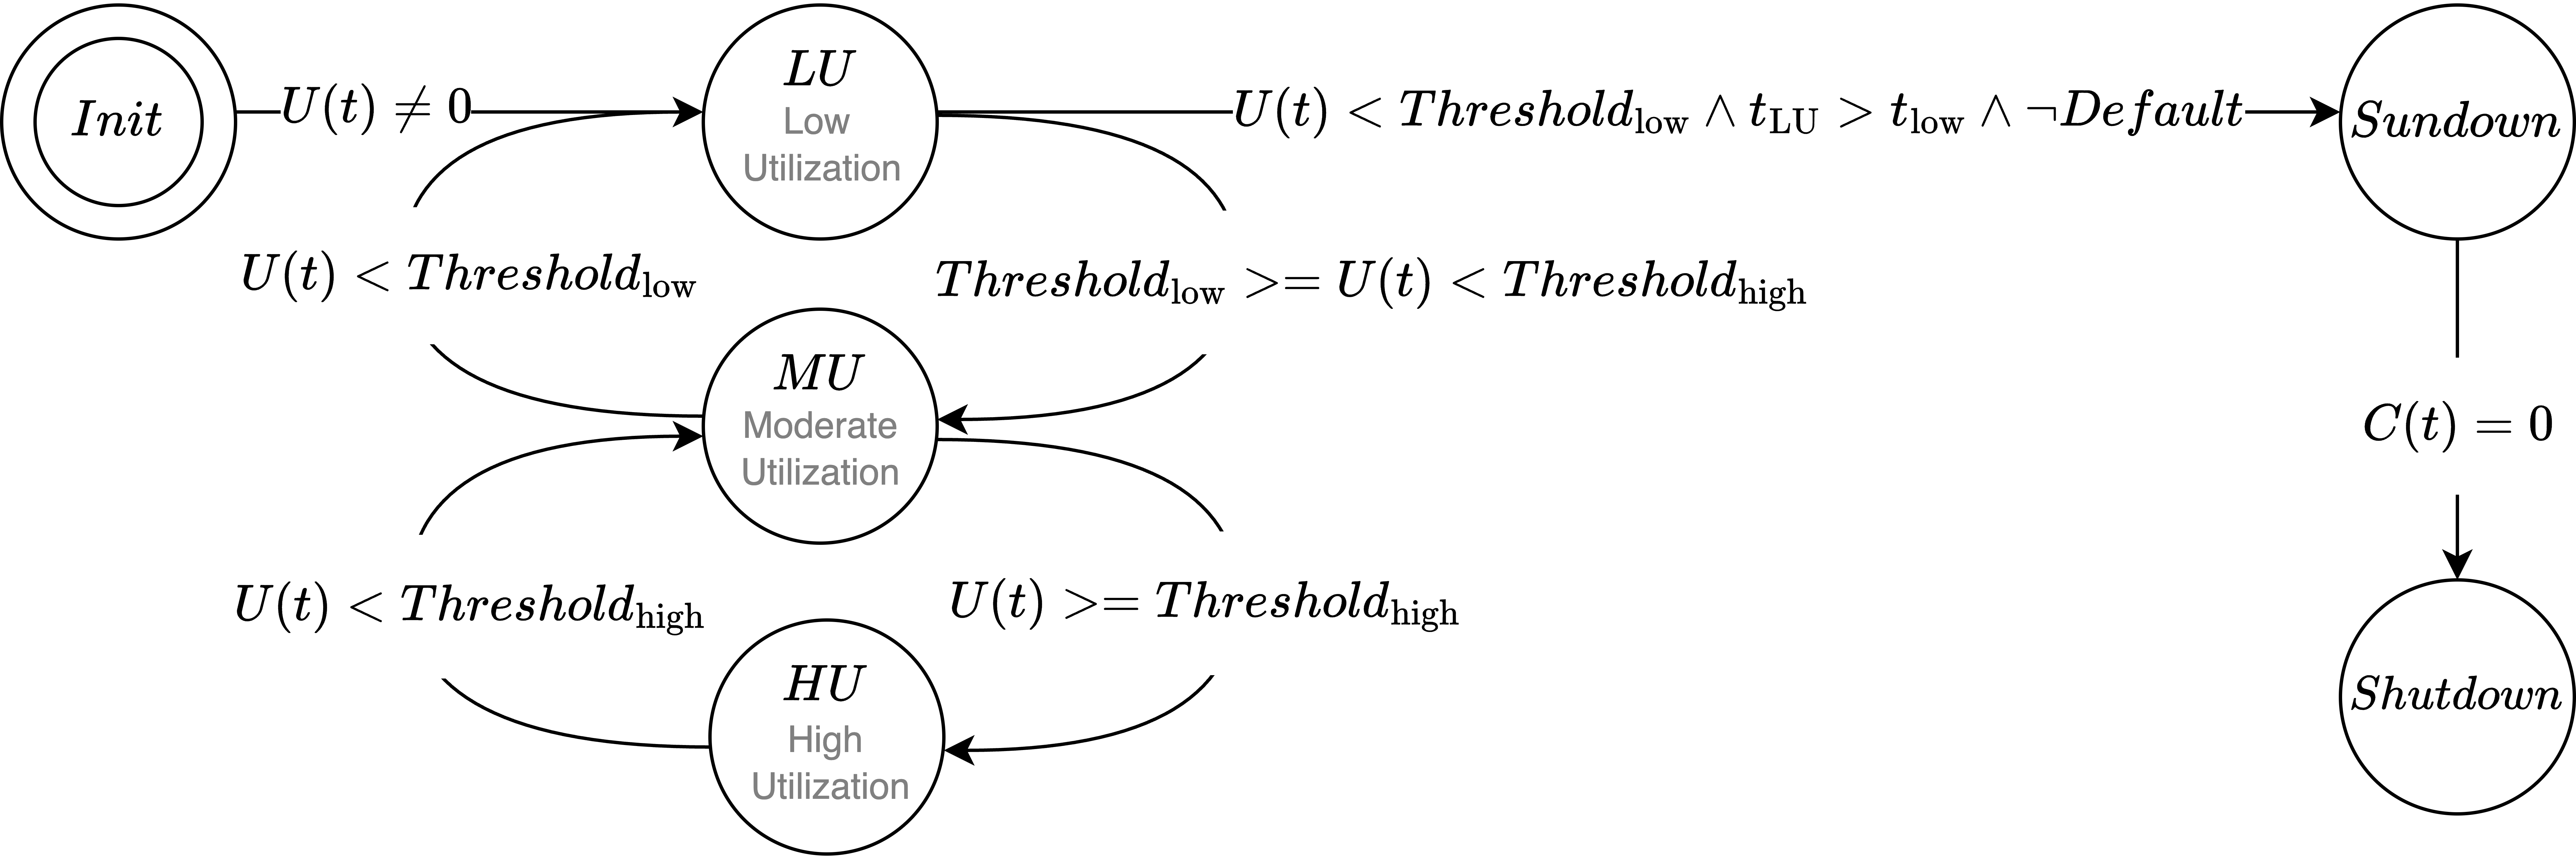
\includegraphics[width=\textwidth]{utilizations.drawio.png}
    \caption{Finite state automaton illustrating worker state transitions based on workload levels. Transitions are governed by thresholds $Threshold_{low}$ and $Threshold_{high}$, with a hysteresis mechanism to prevent unnecessary reallocations. The final shutdown occurs when active connections $C(t)$ reach zero.}
    \label{fig:automat}
\end{figure*}

\subsection{Distribution of scores}
The \textit{Balancer} requires the scores to effectively distribute load according to corresponding utilization. For communication via the socket, a queue is implemented. In information technology, a queue possesses the essential characteristic of determining order based on the First In, First Out principle\cite{black2020queue}. In the context of the described load balancer, the queue \( Q \) represents an ordered data structure comprising elements \( (Q_i, s_i) \), where \( Q_i \) denotes the element and \( s_i \) its associated score. This queue exhibits a dynamic size, allowing it to accommodate any number of elements as needed. Formally, we can define a queue as a set:
$$Q = \{ (Q_1, s_1), (Q_2, s_2), \dots, (Q_n, s_n) \}, \quad n \in \mathbb{N}$$
In this representation, \( n \) signifies the number of elements within the queue, which can grow arbitrarily large. The queue undergoes both periodic generation and querying processes. The queue grows as the system, specifically the \textit{Deployment-Agent}, scales multiple containers, thereby altering the pairs within the queue. Theoretically, a queue can contain an infinite number of \textit{Workers}, although in practice, system resources limit its size. In practical implementation, the queue within the Load Balancer initializes and contracts to the configured default number of \textit{Workers}, and scales up to the configured upper limit. Additionally, in the actual implementation, the queue also sends the utilization category for each container, derived from the calculated score \( s_i \). This category will be explained in the next subchapter.

\subsection{Worker utilization}
The algorithmic approach involves transforming numerical scores into utilization categories, a process designed to enhance interpretability. This reduction of continuous scores into discrete categories (Low, Medium, High Utilization) significantly eases data interpretation. This approach is grounded in the psychological principle of cognitive load, which insists that humans more readily process and comprehend discrete categories compared to continuous valuesn\cite{cogload}. Moreover, this categorization method offers an inherent buffer against minor measurement fluctuations, providing a degree of error tolerance in the analysis. The algorithm for the transition between the states of a \textit{worker} can be explained using the finite automaton depicted in Figure~\ref{fig:automat}. The presented model is based on a stochastic finite automaton representing different workload levels. The state transitions are controlled by a multidimensional evaluation function, whose thresholds $Threshold_{low}$ and $Threshold_{high}$ are based on empirical data from large cloud providers like Azure Autoscale\cite{azure_autoscale_best_practices}, but can also be modified in the application configuration afterward. A central element of the model is the Sundown state, defined by \( P(LU \rightarrow Sundown) \) as:
$$P(U(t) < Threshold_{low} \wedge t_{LU} > t_{low} \wedge \neg Default) $$
This state implements a hysteresis mechanism that distinguishes short-term load fluctuations from long-term trends, thus preventing unnecessary resource reallocations. The transition to the final shutdown state is governed by the condition $C(t) = 0$, where $C(t)$ represents the cardinality of the set of active connections at time $t$. The differentiation between default and non-default workers leads to a conditional termination property:

$$ \forall w \in W: T(w) = \begin{cases}
                               0 & \text{if } w \in D \\
                               1 & \text{if } w \notin D
\end{cases} $$
Here, $W$ represents the set of all workers, $D \subset W$ the subset of default workers, and $T(w)$ the termination function. This distinction enables fine-grained control over system stability and scalability. The model addresses the challenges of dynamic load balancing in microservice architectures and provides a theoretical framework for implementing adaptive orchestration strategies. Elements of queueing theory are applied in the analysis of connection states and resource request management, particularly where the consideration of $C(t)$ shows parallels to M/M/c queueing models. Additionally, it integrates aspects of the Markov decision process, especially in the modeling of state transitions, allowing a probabilistic view of the system dynamics\cite{kendall1953stochastic}. This enables the system to maintain an optimal balance between resource efficiency and service availability. The consideration of connection states and worker classification allows for fine-grained control over resource allocation, which is particularly important in highly scalable, containerized infrastructures.

\subsection{Scaling}
Building on the finite automatom previously introduced (Figure~\ref{fig:automat}), the process of scaling containers up and down can now be described. The system’s decision to launch a new \textit{worker} is modeled by state transitions, which are triggered by predefined threshold values. These transitions are governed by configurable variables. Specifically, \( C_{\text{running}}(t) \) denotes the number of active containers at time \( t \), while \( C_{\text{default}} \) represents the minimum predefined number of containers, and \( C_{\text{max}} \) represents the maximum allowable number of containers. Both values are configurable. As previously discussed, \( U(t) \) represents the system utilization at time \( t \), which is calculated based on the corresponding performance scores.

\subsubsection{Scale-up (container start-up)}
The process of scaling up new containers is triggered when the system load exceeds certain thresholds and the current number of containers is below the maximum limit. Let $C(t)$ be the number of active containers at time $t$, $L(t)$ be the average system load, and $L_c$ be the load of an individual container $c$. The conditions for scaling up are $C(t) < C_{\text{max}}$ and $L(t) < L_{\text{high}} \quad \text{or} \quad \min(L_c) < L_{\text{critical}}$ Where $C_{\text{max}}$ is the maximum number of allowed containers, $L_{\text{high}}$ is the high load threshold, and $L_{\text{critical}}$ is the critical load threshold for individual containers. When these conditions are met, the system scales up by adding new containers: $C(t+1) = \min(C(t) + S, C_{\text{max}})$. Where $S$ is the scaling step (number of containers to add in one operation).

\subsubsection{Scale-down (container shutdown)}
The process of scaling down containers is initiated when the average system load exceeds a low threshold while the number of active containers is above the default minimum. This can be represented as: $\bar{L}(t) > L_{\text{low}} \quad \text{and} \quad C_{\text{active}}(t) > C_{\text{default}}$ Where $\bar{L}(t)$ is the average load, $L_{\text{low}}$ is the low load threshold, $C_{\text{active}}(t)$ is the number of active containers, and $C_{\text{default}}$ is the default minimum number of containers. When these conditions are met, containers are marked for graceful shutdown (Sundown state): 
$C_{\text{sundown}}(t+1) = \min(S_{\text{step}}, C_{\text{active}}(t) - C_{\text{default}})$ Where $S_{\text{step}}$ is the scaling step and $C_{\text{sundown}}$ is the number of containers marked for Sundown. The system then updates the default container count: $C_{\text{default}}(t+1) = \max(C_{\text{default}}(t) - C_{\text{sundown}}(t+1), C_{\text{env\_default}})$. Where $C_{\text{env\_default}}$ is the environment-defined minimum number of containers.

\subsubsection{Cooldown Periods}
In addition to the above conditions, a cooldown period \( T_{\text{cooldown}} \) is defined to ensure that a minimum amount of time \( t_{\text{elapsed}} \) has passed between two scaling actions. This condition can be expressed as:
\[
    t_{\text{elapsed}} \geq T_{\text{cooldown}}
\]
During the cooldown period, no scale-up or scale-down actions are performed, thereby preventing excessive start-stop cycles that could negatively impact system stability.
\subsection{Load Distribution Model}
The Dynamic Weighted Load Balancer is based on the principle of weighted random selection, modeled by a discrete probability distribution. Let \( \mathcal{S} = \{s_1, \ldots, s_N\} \) be the set of available servers and \( \mathcal{W} = \{w_1, \ldots, w_N\} \) their corresponding weights. The probability \(  p_i \) that server \( s_i \) is selected is defined as:
$$
p_i = \frac{w_i}{\sum_{j=1}^N w_j}, \quad i = 1, \ldots, N
$$
This distribution corresponds to a categorical distribution with parameter \(\mathbf{p} = (p_1, \ldots, p_N)\). For the load model, let \(R\) be the total number of requests. The expected number of requests \(r_i\) for server \(s_i\) follows the distribution \( (r_1, \ldots, r_N) \sim \text{Multinomial}(R, \mathbf{p}) \) with the theoretical expected value of:
$$
\mathbb{E}[r_i] = R \cdot p_i = R \cdot \frac{w_i}{\sum_{j=1}^N w_j}
$$
To assess the efficiency of this distribution, two scenarios are compared. The following efficiency metric is used for comparison, defining the efficiency \(\eta\):
$$
\eta = \frac{\min_{i} \{r_i / w_i\}}{\max_{i} \{r_i / w_i\}}
$$
Two contrasting scenarios with \(N = 4\) servers and \(R = 10^4\) requests are examined.

\subsubsection{Approximation of Heterogeneous Loads}
With a load of \(\mathcal{W}_1 = \{100, 50, 25, 5\}\), the theoretical load distribution is \( \mathbb{E}[r_i] = (5556, 2778, 1389, 278)\). With a simulated distribution of \((5600, 2700, 1400, 300)\), the result is:
$$\eta_1 = \frac{\min \{56, 54, 56, 60\}}{\max \{56, 54, 56, 60\}} = 0.9$$

\subsubsection{Approximation of Homogeneous Loads}
With a more balanced load of \(\mathcal{W}_2 = \{100, 95, 90, 85\}\), the theoretical distribution is \(\mathbb{E}[r_i] = (2700, 2570, 2430, 2300)\). With a simulated distribution, the result is:
$$
\eta_2 = \frac{\min \{27.2, 26.84, 27.22, 26.82\}}{\max \{27.2, 26.84, 27.22, 26.82\}} \approx 0.985
$$


\subsubsection{Measurement Data Collection}
In order to empirically validate the theoretical framework, measurement data was collected based on the \textit{workers}, scores, and utilization categories. The programmatic components for calculating the weights based on the probability model were implemented using a function that generated random queues. The execution cycle of the program first instantiated a queue, calculated the weights based on the random scores, and subsequently updated the statistics of the \textit{workers} for the following iteration. It is important to note that this data collection method represents a worst-case scenario for heterogeneous utilization, as the fluctuation range of incoming queues per time-based distribution iteration is significantly more varied in real-world conditions. The script used for generating the measurement data was executed 100 times, with minor delays introduced between each simulation run. The simulation itself, similar to the actual implementation, adhered to identical temporal intervals. The visual representation of the data obtained from the simulation resulted in the following graphical model:
\begin{figure}[htbp]
    \centering
    \begin{tikzpicture}
        \begin{axis}[
        width=\columnwidth,
        height=7cm,
        xlabel={Time (s)},
        ylabel={Utilization (\%)},
        ylabel style={at={(axis description cs:0.1,.5)}, anchor=south},
        xmin=0, xmax=33.5,
        ymin=0, ymax=65,
        xtick distance=5,
        ytick distance=10,
        grid=major,
        cycle list name=color list,
        ]

        \addplot[thick] table[x index=0, y index=1, col sep=tab] {data.txt};
        \addplot[thick] table[x index=0, y index=2, col sep=tab] {data.txt};
        \addplot[thick] table[x index=0, y index=3, col sep=tab] {data.txt};
        \addplot[thick] table[x index=0, y index=4, col sep=tab] {data.txt};
        \end{axis}
    \end{tikzpicture}
\end{figure}

\subsubsection{Interpretation}
The analysis demonstrates that the Dynamic Weighted Load Balancer achieves high efficiency in both theoretical scenarios. In the heterogeneous case (\(\eta_1 = 0.9\)), despite significantly varying server capacities, an almost optimal relative load distribution is achieved. In the homogeneous case (\(\eta_2 \approx 0.985\)), efficiency approaches the theoretical maximum of 1. As for the evaluation of the collected data, it can initially be examined in the following time series. Based on the graphical evaluation, the measured data can be considered valid. Each graph exemplifies a single \textit{worker}. The weights are updated based on a new queue at times \(t=2\), \(t=4\), and so on. What is particularly noticeable is how, after a period of high load for a \textit{worker}, the probability of being assigned new loads decreases significantly when utilization exceeds \(50\%\), allowing the \textit{worker's} load to recover swiftly. This recovery ensures that the \textit{worker} is ready and available for new loads in the next cycle. Further interpretation reveals that the load oscillates around the theoretical ideal state. A perfect load distribution would be characterized by a constant straight line, ideally as low as possible on the Y-axis. However, this ideal state is unattainable due to the various variables and environmental factors involved. Each \textit{worker} handles a variable load—code on which the load can be distributed. These requests differ in nature. We can distinguish between human-generated requests, such as a person (user \(w\)) accessing a webpage or service \(x\), and machine-generated requests, where server \(y\) calls server \(z\). Both types of requests share a common feature: the variability in the nature of the requests inherently causes the workers' utilization to fluctuate, for example, due to differing payloads. Additional external factors, such as network speed, contribute to these fluctuations. The variability is even greater with human-generated requests, as they can be interrupted at unpredictable times. All of these factors make a linear distribution impossible. Consequently, load distribution that adapts to varying loads necessarily results in oscillations. This partially answers the question as to why such overhead in load balancing is justified. A comparison with a traditional round-robin algorithm, which introduces virtually no overhead\cite{arpaci-dusseau2014operating}, reveals that in an ideal scenario—where requests arrive at regular intervals, finish simultaneously, have identical payloads, and all participants are equally available—round-robin would indeed result in perfect load distribution. However, as previously discussed, real-world conditions deviate significantly from this ideal. In a worst-case scenario, a worker with extremely high utilization could coexist alongside another worker with almost no utilization, yet both would receive the same load. This justifies the overhead introduced by dynamic load balancing, as it enables the system to continuously adapt and recalibrate, regardless of how extreme or uncertain the incoming requests may be.

\section{Cache}
Especially in the discipline of performance, caching plays a significant role but is complex to integrate with changing requirements\cite{hennessy2011computer}. A distinction is made between static and dynamic caching. Dynamic caching completely changes the caching model and enables the caching of a much broader range of content, including highly dynamic web pages\cite{cloudflare2024caching}. In the described system, a minimalistic static cache is used, which stores entries to reduce latency for frequently requested data and to decrease the number of backend queries. The cache is designed to have a predetermined capacity and entries are removed based on their expiration time (TTL). This implementation contributes to increasing the efficiency of the system by automatically deleting old or rarely used data. The cache is based on the \textit{Rust} data structure \texttt{VecDeque}, a double-ended queue that allows adding or removing entries at both the beginning and the end in O(1) time\cite{rust_vecdeque}. This is particularly useful when the cache reaches its capacity and the oldest entry needs to be removed. The cache entries consist of three components: the key \( k_i \), the cache value to be stored \( v_i \), and the expiration date \( t_i \).We formally define the cache as a set \( C \) containing \( N \) entries:
\[
    C = \{ (k_1, v_1, t_1), (k_2, v_2, t_2), \dots, (k_N, v_N, t_N) \}
\]
The cache operates with a TTL (Time-to-Live) strategy, where each entry \( (k_i, v_i, t_i) \) remains in the cache only until \( t_i \), the expiration time, is reached. If the current time \( t_{\text{now}} \) is greater than \( t_i \), the entry is removed. To remove expired entries, the cache includes garbage collection that runs regularly in a background process. This process checks all entries at certain time intervals \( \Delta t \) to remove outdated entries and efficiently use memory.

\subsection{Access Operations}
When retrieving a value from the cache, it is checked whether the entry is still valid. If the entry has expired, it is removed, and the cache returns \texttt{None}. Otherwise, the cached value is returned. When storing a new entry, it is first checked whether the cache is full. If this is the case, the oldest entry is removed before the new entry is added.

\subsection{Effects on System Performance}
The cache reduces the number of backend requests and optimizes resource utilization. The hit rate \( H \) describes the proportion of requests that can be answered directly in the cache:
\[
    H = \frac{N_{\text{hit}}}{N_{\text{total}}}
\]
A higher hit rate leads to improved overall system performance, as fewer requests need to be forwarded. At the same time, the cache minimizes latency in responding to requests, which is crucial especially in highly scalable environments\cite{tanenbaum2007distributed}.

\section{Request Management}
A request in this system represents an HTTP redirection to one of the \textit{Workers}, implemented using an asynchronous approach. The core of the implementation revolves around the concept of Unbounded-Clients, which leverage \textit{Rust}'s asynchronous high-capacity channels to theoretically allow an unlimited number of concurrent requests. In practice, however, the number of simultaneous requests is constrained by other bottlenecks in the network communication layers. Notably, during extreme load tests of the load balancer at 10,000 requests per second, the connection handling within the business logic of the \textit{Workers'} applications consistently reached its limit before the request management system. A test scenario where the request management system itself became the limiting factor could not be reproduced. Nevertheless, the configuration allows for setting an artificial limit on the number of requests. A crucial aspect of the implementation is the integration of an implicit backpressure mechanism through the use of an mpsc (Multiple Producer, Single Consumer) channel. This mechanism, conceptually aligned with the work of Abdelzaher et al. (2003) on performance control in software services, ensures adaptive load regulation, thereby preventing potential system overloads\cite{backpressure}. The system's robustness is further enhanced by a comprehensive error handling system and a timeout mechanism. Moreover, the implementation addresses concurrency challenges by utilizing Arc (Atomic Reference Counting) for thread-safe access to shared resources. The fundamental process of handling a request can be described as follows: When a request \( r_i \) enters through the external port of the \textit{Balancer} (Figure~\ref{fig:minimal}), it is placed as the \( i \)-th request at time \( t_i \) within the queue. Each worker thread then retrieves a request from the queue and executes it, represented as \( \text{Worker}_k(r_i) \rightarrow \text{Result}(r_i) \). The total latency for a request is the sum of its queuing time and processing time by the worker.

\section{Network Communications}
The foundation of the network architecture is a dedicated \textit{Docker} network based on the bridge driver. This configuration creates an isolated network environment for the containers while enabling efficient communication between system components. The choice of a bridge network offers several advantages: it ensures isolation between containers and the host system while allowing controlled communication\cite{docker_bridge_network}. Container identification and localization within the network is accomplished through a DNS-based system. Each container is assigned a unique name upon creation, which functions as a DNS name within the \textit{Docker} network. The generation of these names is based on a UUID system, ensuring an extremely low probability of collisions\cite{uuid}. Communication between system components occurs via two primary protocols: WebSocket for real-time updates and HTTP for RESTful interactions. The WebSocket connection enables bidirectional, event-based communication with low latency, which is particularly important for dynamically updating the load balancer status. HTTP connections primarily serve for system status queries and configuration. This network architecture facilitates a robust, scalable, and efficient communication infrastructure. The isolation provided by the \textit{Docker} network enhances security, while the DNS-based naming system simplifies service discovery and inter-container communication. The combination of WebSocket and HTTP protocols allows for both real-time responsiveness and traditional request-response interactions, catering to various operational needs of the system.

\section{Redis as State Storage}
In the present implementation of the load balancing system, \textit{Redis} plays a critical, albeit specialized, role. Unlike many typical use cases, \textit{Redis} here does not serve as a comprehensive state storage or communication medium, but primarily as an efficient key-value store for container states and their metadata. \textit{Redis} stores a dataset for each container, identified by an MD5 hash-based key. This dataset includes essential information such as the container's category, numeric score, assigned port, and the Docker image used. The choice of \textit{Redis} for this task is based on its high read and write speed for simple data structures.
In a system requiring constant updates of container status, \textit{Redis} offers significant performance advantages with an average access time of <1ms\cite{redis_docs}. In the main application, \textit{Redis} is initialized at system startup, enabling system state recovery after restarts or failures. This is crucial for maintaining system consistency in dynamic environments. A key aspect is the storage and management of the configuration for default containers, previously mentioned as \( C_{\text{default}} \). This is stored not only in the environment variable but also in \textit{Redis}, allowing for dynamic adjustment of the system configuration at runtime. Moreover, two critical scenarios are addressed: the presence of local containers without corresponding database entries and vice versa. The latter would be the case in the event of an unexpected crash of one of the \textit{Workers}. The synchronization process begins with retrieving currently running containers. Simultaneously, all container entries stored in \textit{Redis} are retrieved. The reconciliation of these two datasets is accomplished by creating a HashSet of the running container keys. For each container entry present in the database, it is checked whether a corresponding running container exists. If not, the database entry is considered obsolete and deleted. This cleanup ensures that the database does not contain entries for no longer existing containers, preventing erroneous decisions in the load balancing process. Conversely, new entries are created for all running containers that do not have a corresponding database entry. This bidirectional synchronization process ensures that the state stored in \textit{Redis} always accurately represents the actually running containers. This approach leverages \textit{Redis}'s strengths in fast data retrieval and storage, while implementing a robust synchronization mechanism that maintains system integrity even in the face of unexpected events or system restarts.

\section{Classification In the context of the online load balancing problem}
The Online Load Balancing Problem addresses the task of distributing incoming jobs in real-time across available resources (typically servers) without prior knowledge of future jobs. In a formal definition, let \( M = {m_1, ..., m_n} \) be the set of available machines, and \( J = {j_1, ..., j_m} \) the incoming jobs, where each job $j_i$ has a processing time $p_i$. The most common solution to this problem is the Greedy algorithm, which assigns each job to the least loaded machine\cite{black2020greedy}. This approach was improved by Azar et al, who randomly assign each job to two machines and then choose the less loaded one\cite{AZAR199473}. This improved the competitiveness of the Greedy algorithm from $O(n)$ to $O(\log \log n)$. To demonstrate the efficiency of the presented implementation, we assume there are 1000 tasks to be distributed. Efficiency is measured by the maximum load on a single \textit{worker} (also known as makespan). The complexity of distribution in the implementation stems from the dynamic generation of scores to weights within the \textit{Balancer}. The sampling itself would only cost $O(1)$, but since weights are reconstructed with each significant change, it becomes $O(\log n)$. Additional factors include updating weights from the queue, which is performed periodically and asynchronously, thus less frequently, with $O(n)$. Assuming a perfect distribution would lead to a maximum load of 100 units per server, then $C_{OPT}(n)$ would be the optimal solution. Thus, the costs for the implementation would comprise $C_{OPT}(n) + O(\log n)$. However, it must be considered that due to periodic queue updates, there is always a configurable delta where performance deviates from the optimum. The deviation is smallest immediately after an update and largest just before the next update. $\Delta(t)$ is the time-dependent deviation from the optimum (0 ≤ t < 2 seconds, value in the default configuration). This would result in an approximation of the complexity with $C_{OPT}(n) + O(\log n) + \Delta(t)$. From this, it can be deduced that the algorithm presented here offers a good compromise between performance and adaptivity, but requires particular attention in fine-tuning the update frequency to fully exploit its advantages. The dynamic weighting is superior to the two compared algorithms but has disadvantages in an absolute worst-case scenario with high volatilities of utilization if $\Delta(t)$ should be chosen too large. Regarding scalability for very large $n$, the demonstrated algorithm closely follows Azar, and both are far ahead of Greedy ($O(\log \log n) < O(\log n) < 2 - 1/n$).


\section{Conclusion}
The presented implementation of an online load balancing system marks a contribution to bridging the gap between theoretical models and practical applications in the field of distributed systems. By utilizing \textit{Rust} and \textit{Docker}, this approach opens up new possibilities for scalable and efficient load distribution across a variety of application scenarios. The system's flexibility, particularly its ability to dynamically adapt to heterogeneous load conditions, makes it a promising candidate for deployment in edge computing environments, where resource constraints and fluctuating network conditions are common occurrences. Future research could focus on integrating machine learning techniques to enhance the system's predictive capabilities and enable proactive load distribution decisions. This could prove especially valuable in environments with predictable load spikes, such as those experienced by e-commerce platforms during sales events. Furthermore, extending the system with energy optimization features could transform it into a valuable tool for green computing initiatives, optimizing load distribution not only for performance but also for energy efficiency. The open nature of the implementation invites collaboration and further development, potentially leading to a robust ecosystem of extensions and adaptations. This could pave the way for standardized, open-source load balancing solutions capable of competing with proprietary systems. Ultimately, this work demonstrates that practice-oriented research in the field of distributed systems not only holds academic value but can also have direct and significant impacts on the development of real-world, high-performance infrastructures.

\bibliography{references}




\end{document}

% end of file template.tex
%%%%%%%%%%%%%%%%%%%% TeXStudio Magic Comments %%%%%%%%%%%%%%%%%%%%%
%% These comments that start with "!TeX" modify the way TeXStudio works
%% For details see http://texstudio.sourceforge.net/manual/current/usermanual_en.html   Section 4.10
%%
%% What encoding is the file in?
% !TeX encoding = UTF-8
%% What language should it be spellchecked?
% !TeX spellcheck = en_US
%% What program should I compile this document with?
% !TeX program = pdflatex
%% Which program should be used for generating the bibliography?
% !TeX TXS-program:bibliography = txs:///bibtex
%% This also sets the bibliography program for TeXShop and TeXWorks
% !BIB program = bibtex

%%% Local Variables:
%%% mode: latex
%%% TeX-master: t
%%% End:
